%\VignetteIndexEntry{PKreport Overview}
%\VignetteDepends{PKreport}
%\VignetteKeywords{PKreport}
%\VignetteKeywords{PKreport}
%\VignetteKeywords{PKreport}
%\VignettePackage{PKreport}
\documentclass[a4paper]{article}

\newcommand{\Rfunction}[1]{{\texttt{#1}}}
\newcommand{\Robject}[1]{{\texttt{#1}}}
\newcommand{\Rpackage}[1]{{\textit{#1}}}
\newcommand{\Rclass}[1]{{\textit{#1}}}
\newcommand{\Rmethod}[1]{{\textit{#1}}}

\author{Xiaoyong Sun$^\dagger$$^\ddagger$\footnote{johnsunx1@gmail.com}}

\usepackage{Sweave}
\begin{document}

\setkeys{Gin}{width=1\textwidth}

\title{User Guide for PKreport Package}
\maketitle
\begin{center}$^\dagger$Bioinformatics and Computational Biology Program, $^\ddagger$Department of Statistics \\ Iowa State University, Ames, Iowa 50010, USA
\end{center}

\tableofcontents
%%%%%%%%%%%%%%%%%%%%%%%%%%%%%%%%%%%%%%%%%%%%%%

\section{Introduction}

Graphics play an important and unique role in population pharmacokinetic (PopPK) model building by exploring hidden structure among data before modeling, detecting extremity during modeling, and validating results after modeling. However, to our knowledge there are no tools available to provide an automatically pipeline for routine graphic generation and it also requires users to have expertise in statistical and computing knowledge to generate all related graphics. This may provide obstacles to users who do not have this expertise. In this work, I developed an automatically pipeline, an R package called PKreport, for testing model assumptions, visualizing data and diagnosing models. PKreport aims to 1) provide automatic pipeline for users to visualize data and models. It creates a flexible R framework with automatically generated R scripts to save time and cost for later usage; 2) implement an archive-oriented management tool for users to store, retrieve and modify figures. 3) offer powerful and convenient service to generate high-quality graphs based on two R packages: lattice and ggplot2. The general architecture, running environment and statistical methods can be easily extended to include more automatic diagnostics in the development of PopPK models.

\section{Installation}
You can install PKreport with the following command,
\begin{verbatim}
install.packages("PKreport")
\end{verbatim}
For users who do not have administrative privilege for their computers, they can install this package in their own accounts:\begin{verbatim}
install.packages("PKreport", lib.loc="User directory")
library("PKreport", lib.loc="User directory")
\end{verbatim}

\section{Software implementation}

PKreport is one R package aiming to create an automatic pipeline for model assumption testing. Based on a hidden metric system matching default variables to data variables, this package turns the assumption testing to a fast, convenient and comprehensive routine. With the support of two powerful R graphical packages (\textit{lattice} and \textit{ggplot2}), this software can generate high-quality figures for further diagnosing, archive all figures with specific folders for report and review, and utilize web browsers as interface for viewing, archiving and analyzing.

\subsection{Metric system}

The default variables function as currency for communicating between data sets and packages to generate special-purpose plots (Table~\ref{c2_s3_t1}). For example, PRED represents prediction calculated from nonlinear mixed effects model fitting, and RES is equal to the difference between observations and predictions. Users may use preferred software to calculate these related variables. As a result, each data set and fitting results have totally different variable names for further analysis. To facilitate model diagnostics, users need to match the default metric with the variables from data sets. After matching, the package can process the data, configure the functions, and generate related diagnostic plots. This system provides ways to function for diverse software such as NONMEM, Monolix, R nlme package, and SAS NLMIX procedure.

\begin{table}[h!tb] \centering
% Use: \begin{tabular{|lcc|} to put table in a box
\begin{tabular}{lcc} \hline
\textbf{Package variable} & \textbf{Description}  \\ \hline
ID & Patient ID \\
TIME & Time after dose \\
CONC & The concentration of drug in the body \\
PRED & Prediction generated from model fitting \\
RES & Residual \\
WRES & Weighted residual \\
IPRED & Individual prediction \\
IWRES & Individual weighted residual \\
COV & Covariates \\ \hline
\end{tabular}
\caption{Package metric system. The first column (Package variable) contains default variable names. These default variable names match NONMEM naming system. The second column explains the details of these variables.}
\label{c2_s3_t1}
\end{table}

\subsection{Configuration}

The whole system is configured by three lists: 1) graph list. This list helps user to choose proper figure format (jpg, pdf, png, etc.) as well as the graphical packages. Currently there are two graphical packages implemented for high-quality figures (\textit{lattice} and \textit{ggplot2}). 2) histogram list. This list specifies the configuration for the histogram generated by package. It includes type of histogram and layout setup. 3) scatterplot list. This list determines the type of scatter plot, bandwidth of smooth and layout setup.

\subsection{Architecture description and features}

Currently PKreport offers console user interface to test model assumptions. It has the following functions: 1) Match metrics. By matching default variables to data variables based on one-to one or one-to-many schema, this function sets up global variables for further analysis. 2). Configure figures. This module determines the figure format, figure size and other related properties of figures. 3). Generate figures. Depending on the research goals, users have access to 7 sub-functions for exploratory data analysis, overall goodness of fit plots, parameter diagnostics, random effect diagnostics, structural model diagnostics, residual model diagnostics, and covariate model diagnostics. Each sub-function will create a folder to store related figures as archives. 4). Display results. PKreport offers web browser as a management tool to explore archives created in function 3 and R scripts in function 5. The main interface includes categories matching the name of file directories. 5). Generate R scripts. To improve
efficiency and help users to generate high-quality figures, users have option to modify
related R scripts to meet their specific requirements. All generated R scripts match the order of figures generated in function 4. 6). Modify figures. Users can also update or modify certain figures with figure ID for particular purpose. 7). Clean archives. This module will delete all archives (file directories and figures) and clean global variables in R environment. The general architecture is shown in Fig.~\ref{c2_s1_1}.

\subsection{Format for input data}

PKreport accepts two types of input data: data.frame or \textit{nonmem} class:

\subsubsection{data.frame as input data}

PKreport accepts data.frame and diagnoses model results from NONMEM, Monolix, R nlme, etc. For NONMEM, the data.frame can be read in R directly from tab file. For Monolix, there are a few output files, and users have to combine them as one single file (demonstrated in example 6). This single file is then read in R as data.frame.

\subsubsection{\textit{nonmem} class as input data}

\textit{nonmem} class is specifically designed for NONMEM. The option \textit{output.lst}, and \textit{ output.dir} is for NONMEM 7. The option \textit{ output.tab} is available for any NONMEM version.

\section{Function description}
This package includes 1 \textit{nonmem} class and 5 main functions:
\begin{itemize}
	\item  \textit{nonmem} class: this S4 class contains all NONMEM output, and users can conveniently have access to each section of output.
	\item PKdata: this function helps user to input data (tab file) into package (first parameter), and match the data variables to the package metric system (second parameter).
	\item PKconfig: this function provides a configuration tool to users for managing global parameters and figure setup. It takes three lists (global.list, hist.list, scatter.list) as parameters.  If no lists are configured, the default configuration will be used.
	\item PKfigure: this function is the main interface for generating reports.
  It takes three components: data from NONMEM tab file, diagnostic methods (described in the following
  section), and a logical value to keep or delete previous PKfigure run.
	\item PKshow: this function will open web browser, load all results and generate reports.
	\item PKclean: this function will delete all folders and figures generated for the reports.
\end{itemize}

\subsection{\textit{nonmem} class}
\subsubsection{Slots in \textit{nonmem} class}
This class includes the following slots:
\begin{itemize}
	\item file.cov: a list, includes title (character) and data (data.frame) for cov file.
	\item file.cor: a list, including title (character) and data (data.frame) for cor file.
	\item file.coi: a list, including title (character) and data (data.frame) for coi file.
	\item file.phi: a list, including title (character) and data (data.frame) for phi file.
\item file.lst: a character vector, containing the information from NONMEM lst file.
\item method: a character vector, matching \#METH tag in lst file and containing the estimation method.
\item analysis: a list, matching text between \#TERM tag and \#TERE tag in lst file and contains the analysis information.
	\item objt: a character vector, matching \#OBJT tag in lst file and describes the objective function.
	\item objv: a character vector, matching \#OBJV tag in lst file and describes the objective function value.
	\item objs: a character vector, matching \#OBJT tag in lst file and describes the objective function standard deviation.
\item tabid: a character vector, from the first line of tab file and describes the title of tab file
\item tabdata: a data frame, matching data in tab file and describes the title of tab file. This is the main data for PKfigure.
\end{itemize}
nonmem instances are created through \textit{new("nonmem", ...)}.
The arguments to \textit{new} should include output.lst and output.tab.
If output.dir is missing, NULL will be assigned to proper slots.
The option \textit{output.lst}, and \textit{ output.dir} is for NONMEM 7. The option \textit{ output.tab} is available for any NONMEM version.
\begin{verbatim}
> myclass <- new("nonmem", output.lst="C:/nonmem7/KAKOE.lst",
               output.tab="C:/nonmem7/KAKOE.FITKAKOEST_PAR.FIT",
               output.dir="C:/nonmem7")

\end{verbatim}

\subsubsection{Methods in \textit{nonmem} class}
This class includes the following methods:
\begin{itemize}
	\item non.cov: return file.cov slot.
	\item non.cor: return file.cor slot. 
	\item non.coi: return file.coi slot.
	\item non.phi: return file.phi slot.
\item non.lst: return file.lst slot.
\item non.lst.meth: return method slot, matching \#METH tag in lst file and containing the estimation method.
\item non.lst.term: return analysis slot, matching text between \#TERM tag and \#TERE tag in lst file and contains the analysis information.
	\item non.lst.objt: return objt slot, matching \#OBJT tag in lst file and describes the objective function.
	\item non.lst.objv: return objv slot, matching \#OBJV tag in lst file and describes the objective function value.
	\item non.lst.objs: return objs slot, matching \#OBJT tag in lst file and describes the objective function standard deviation.
\item non.tab: return file.tab slot. This is the main data for PKfigure.
\item non.select: return user-specified lines from lst file. If the length of all lines are equal,
	a data.frame is returned; otherwise a list is returned.
\end{itemize}

\begin{verbatim}
> non.lst(myclass)
> non.select(myclass, c(1:5))
> non.select(myclass, c(20:25))
[[1]]
[1] "MDV"  "DATA" "ITEM" "IS"   "DATA" "ITEM" "NO.:" "8"   

[[2]]
[1] "0INDICES"   "PASSED"     "TO"         "SUBROUTINE" "PRED:"     

[[3]]
[1] "9"  "11" "5"  "7"  "0"  "0"  "6"  "0"  "0" 

[[4]]
[1] "0" "0"

[[5]]
[1] "0LABELS" "FOR"     "DATA"    "ITEMS:" 

[[6]]
 [1] "ID"   "PID"  "TAD"  "DV"   "AMT"  "CMT"  "RATE" "MDV"  "EVID" "TIMB" "TIME"
\end{verbatim}

\subsection{PKdata}
This function includes two parameters:
\begin{itemize}
	\item data: a data frame to analyze. Generally it is from tab file generated from NONMEM.
	\item match.term: a list. It matches the package metrics to the variable names in the data. 
	For ID, DV, TIME, PRED, RES, WRES, IPRE, the package only allows one variable to match 
	these terms. Users can use CWRES, NWRES to match WRES based on their research goals. 
	For COV, PARA, ETA, the package accepts multiple variables a character vector.
\end{itemize}


\begin{verbatim}
> head(pdata)
  ID PID    TIME    DV  IPRED    CWRES EVID
1  1   1 0.00000  0.00  0.000  0.00000    0
2  1   1 0.49861  0.00  0.000  0.00000    1
3  1   1 0.49861  0.00  0.000  0.00000    1
4  1   1 0.99917 15.84 12.674  1.49810    0
5  1   1 1.49940 27.20 46.562 -1.69600    0
6  1   1 1.99920 62.90 73.010 -0.57653    0
          TAD    ETA1    ETA2    ETA3 ETA4 ETA5
1 -0.49833000 0.32094 0.16727 0.26971    0    0
2  0.00027778 0.32094 0.16727 0.26971    0    0
3  0.00027778 0.32094 0.16727 0.26971    0    0
4  0.50083000 0.32094 0.16727 0.26971    0    0
5  1.00110000 0.32094 0.16727 0.26971    0    0
6  1.50080000 0.32094 0.16727 0.26971    0    0
      ETA6 ETA7  DV.1   PRED      RES     WRES
1 -0.34748    0  0.00  0.000   0.0000  0.00000
2 -0.34748    0  0.00  0.000   0.0000  0.00000
3 -0.34748    0  0.00  0.000   0.0000  0.00000
4 -0.34748    0 15.84 16.384  -0.5443  0.94749
5 -0.34748    0 27.20 62.534 -35.3340 -1.10160
6 -0.34748    0 62.90 99.985 -37.0850 -0.38250

> var.name <- list(ID="ID", DV="DV", TIME="TIME", PRED="PRED",
                  RES="RES", WRES=c("WRES"),
                  IPRE="IPRED", IDV=c("EVID"),
                  ETA=c("ETA5", "ETA1"), COV="EIVD",
                  PARA=c("ETA2", "ETA3")
                  )

> PKdata(data=pdata, match.term=var.name)
Data is read successfully.
\end{verbatim}

\subsection{PKconfig}
This function includes two parameters:
\begin{itemize}
\item general.list: a list. It includes figure configuration: save.format (png format will be generated automatically as the default format for html report) , width, height, and also graphic packages (0: use only lattice package. 1: use only ggplot2 package. 2: use both packages).
\item hist.list: a list. It includes histogram configuration: type, layout, ind.layout (for individual plots).
\item scatter.list: a list. It includes scatterplot configuration: type, layout, span, ind.layout (for individual plots).
\end{itemize}
This function only supports simple configuration for figures. If you need more complex configuration for figures, please go to R code page in HTML report and regenerate proper figures with those codes.
\begin{verbatim}
> global.list <- list(    save.format=c("jpeg", "bmp"),
                        width = 480, height = 480,
                        package=2
                    )
> hist.list <- list(type=c("count"), layout=c(1,1), ind.layout=c(5,5))
> scatter.list <- list(type=c("p", "smooth"), layout=c(1,1), ind.layout=c(5,5))
> PKconfig(global.list, hist.list, scatter.list)
\end{verbatim}

\subsection{PKfigure}
This function includes three parameters:
\begin{itemize}
	\item data: a data frame to analyze. Generally it is from tab file generated from NONMEM.
\item methods: a numeric vector. It includes all diagnostics methods according to Census,
\begin{itemize}
\item 1: Exploratory data analysis
\item 2: Individual plots
\item 3: Goodness-of-fit plots
\item 4: Structural model diagnostics
\item 5: Residual model diagnostics
\item 6: Parameters diagnostics
\item 7: Covariate model
\item 8: Random effects
\end{itemize}
\item clean: a logical value indicating whether or not to keep results from previous PKfigure for final report.
\end{itemize}
\begin{verbatim}
> PKfigure(pdata, c(1,5,8))
\end{verbatim}

\subsection{PKshow}
This function includes three optional parameter: nonmemObj, a object of class nonmem; 
table.Rowv, a logical value determining whether the row dendrogram should be reordered 
in the heatmap-like table; table.Colv, a logical value determining whether the column 
dendrogram should be reordered in the heatmap-like table.

\begin{verbatim}
# Generate both graphical report and numeric report
> PKshow(myclass, tableRowv=TRUE, tableColv=TRUE)
# Only generate graphical report
> PKshow() 
\end{verbatim}

\subsection{PKclean}
This function is to delete all archives (file directories and figures) and clean global variables in R environment. 
\begin{verbatim}
> PKclean()
\end{verbatim}

\section{Demonstration}
To illustrate how to use this package, five examples are used. 
The first and the second example demonstrate the main functions, 
the third example focuses on the configuration, and the last two examples 
explain the methods related to \textit{nonmem} class.
\subsection{Example 1}
We would like to generate a simple report (only graphical report and no numerical report),
\begin{verbatim}
> data(pdata)
> var.name <- list(ID="ID", DV="CONC", TIME="TIME", 
				  PRED="PRED", RES="RES", WRES="WRES",
                  IDV=c("ISM"), IPRE="PRED",
                  ETA=c("ETA1", "ETA2"), COV=c("WT","AGE"),
                  PARA=c("CL", "V")
                  )
                  
> PKdata(pdata, match.term=var.name)
> PKfigure(pdata, c(3,6,8))
> PKshow()
\end{verbatim}

\subsection{Example 2}
The NONMEM output directory is in \textit{c:\\nonmem7}, and it 
includes lst, tab, cov, cor, coi and phi files. 
We would like to generate a complete report, including both graphical report and numeric report.
\begin{verbatim}
> myclass <- new("nonmem", output.lst="C:/nonmem7/KAKOE.lst",
               output.tab="C:/nonmem7/KAKOE.FITKAKOEST_PAR.FIT",
               output.dir="C:/nonmem7")
> var.name <- list(ID="ID", DV="DV", TIME="TIME", PRED="PRED",
                  RES="RES", WRES=c("WRES"),
                  IPRE="IPRED", IDV=c("EVID"),
                  ETA=c("ETA5", "ETA1"), COV="TIME",
                  PARA=c("ETA2", "ETA3")
                  )

> pdata <- myclass@tabdata
> PKdata(data=pdata, match.term=var.name)

> PKfigure(pdata, 3)
> PKfigure(pdata, 7, FALSE)
> PKshow(myclass, table.Rowv=TRUE, table.Colv=TRUE)
\end{verbatim}

\subsection{Example 3}
We would like to generate report only with R package lattice, and change figure width and height to 500 px.
\begin{verbatim}
> global.list <- list(    save.format=c("jpeg", "bmp"),
                        width = 500, height = 500,
                        package=0
                    )
> hist.list <- list(type=c("count"), layout=c(1,1), ind.layout=c(5,5))
> scatter.list <- list(type=c("p", "smooth"), layout=c(1,1), ind.layout=c(5,5))

> PKconfig(global.list, hist.list, scatter.list)
> PKfigure(pdata, c(3,6,8))
> PKshow(myclass)
\end{verbatim}

\subsection{Example 4}
There are some methods for \textit{nonmem} class. These methods help users to extract specific information from NONMEM output, including estimation method, objective function value, and file contents.
\begin{verbatim}
> non.lst(myclass)
> non.lst.meth(myclass)
[1] "First Order Conditional Estimation with Interaction"
> non.lst.objv(myclass)
[1] "2351.625"
> non.tab(myclass)
> non.cov(myclass)
\end{verbatim}

\subsection{Example 5}
The standard output file (lst file) does not have a tabular format. There are two methods in this packages that can help users to access any line in the lst file. User can check the line number by some text edit software or use \texttt{non.lst} function.
\begin{verbatim}
> non.lst(myclass)
# select lines from 50 to 56 in lst file
> exp.data <- non.select(myclass, c(50:56))
> options(scipen=100)
> PKnum(exp.data)
     [,1]   [,2]       [,3]
[1,]    1  44.80 1000000.00
[2,]    1 410.00 1000000.00
[3,]    0   0.25 1000000.00
[4,]    6  17.00 1000000.00
[5,]    0   0.28 1000000.00
[6,]    0   0.50       0.95
[7,]    0   0.50 1000000.00
> options(scipen=-100)
> PKnum(exp.data)
      [,1]     [,2]    [,3]
[1,] 1e+00 4.48e+01 1.0e+06
[2,] 1e+00 4.10e+02 1.0e+06
[3,] 0e+00 2.50e-01 1.0e+06
[4,] 6e+00 1.70e+01 1.0e+06
[5,] 0e+00 2.80e-01 1.0e+06
[6,] 0e+00 5.00e-01 9.5e-01
[7,] 0e+00 5.00e-01 1.0e+06
\end{verbatim}

\subsection{Example 6}
In the final example, I will demonstrate how to use this package for the output from Monolix. 
These output files are ``predictions.txt'', ``indiv\_eta.txt'', ``indiv\_parameters.txt''.

\begin{verbatim}
# read in Monolix output files
> mpred <- read.table(file.path(
		   paste(system.file("monolix", package="PKreport"), 
		   "predictions.txt", sep="/")),
+          header=T, sep="\t")
> meta <- read.table(file.path(
           paste(system.file("monolix", package="PKreport"), 
		   "indiv_eta.txt", sep="/")),
+          header=T, sep="\t")
> mpara <- read.table(file.path(
		   paste(system.file("monolix", package="PKreport"), 
		   "indiv_parameters.txt", sep="/")),
+          header=T, sep="\t")
> 
# combine three files together as one file
> merge.1 <- merge(mpred, meta, by="ID")
> mdata <- merge(merge.1, mpara, by="ID")
> colnames(mdata) <- gsub("_", ".", colnames(mdata))
> no.index <- which(colnames(mdata) %in% c("X.1", "X.y", "X"))
> mdata <- mdata[, - no.index] 
> 
> PKdata(mdata, match.term=var.name)
Data is read successfully.
> PKfigure(mdata, c(3))
> PKshow()
\end{verbatim}

\begin{figure}[h!tb] \centering
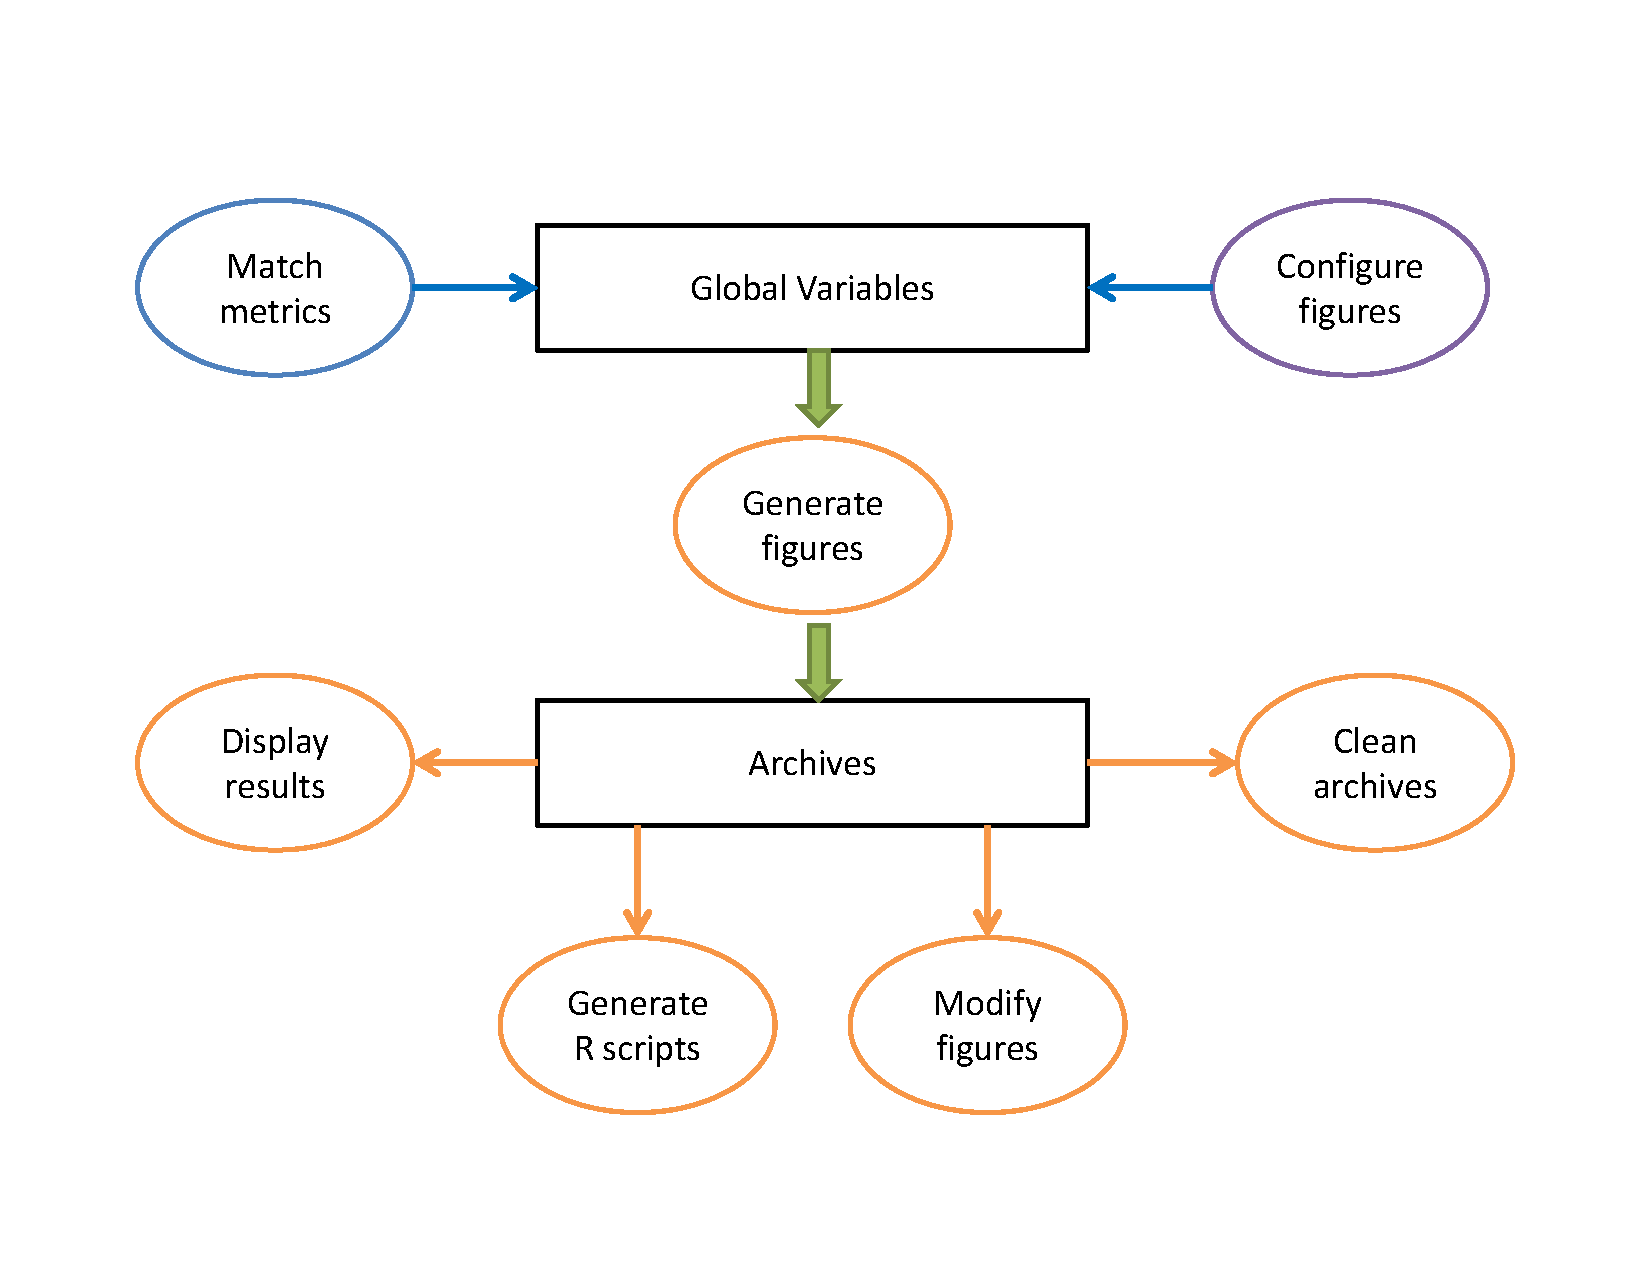
\includegraphics[scale=0.5]{c2_s1_1.pdf}
\caption{Software architecture of PKreport. It has three main functions: 1) match metrics; 2) configure figures; 3) generate figures; 4) display results; 5) generate R scripts; 6) modify figure; 7) clean archives. The first two functions set up working environment, and the other functions help to generate related figures.}
\label{c2_s1_1}
\end{figure}

\begin{figure}[h!tb] \centering
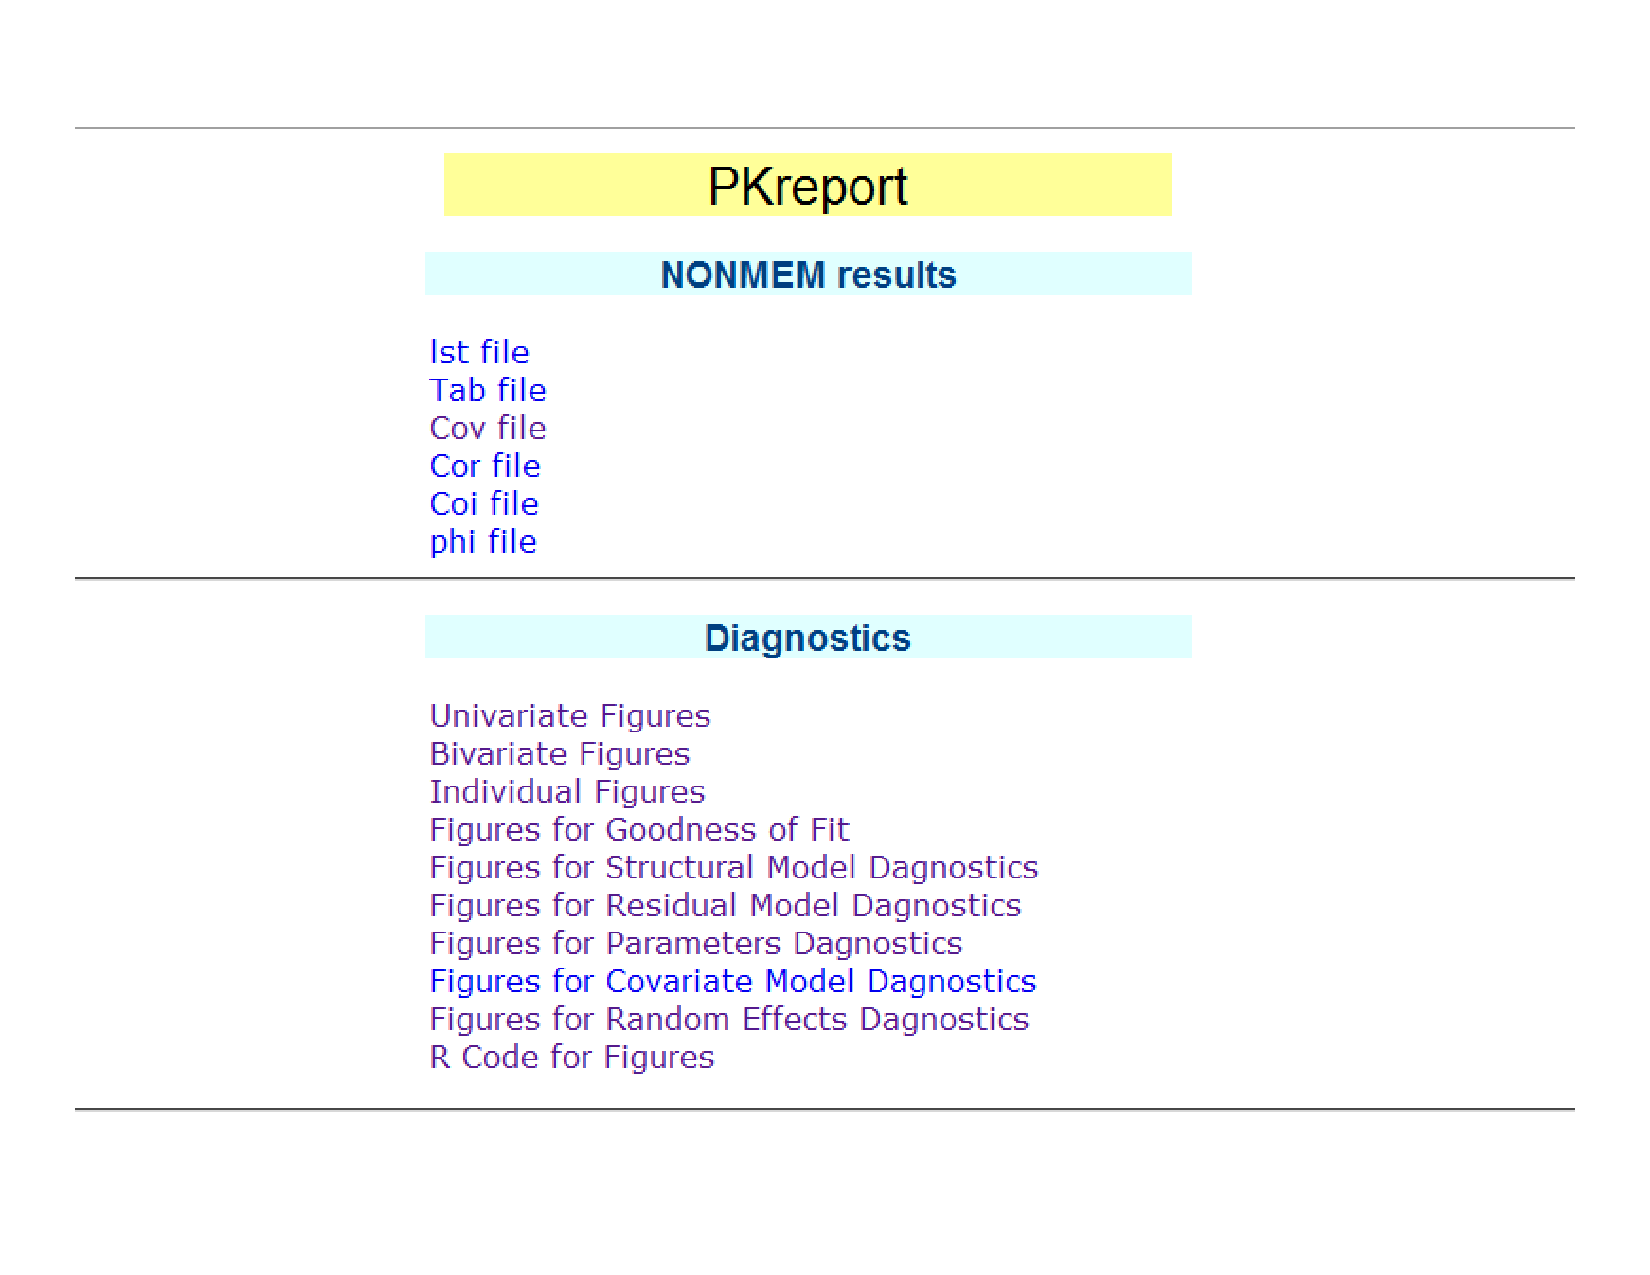
\includegraphics[scale=0.5]{c2_s2_2web.pdf}
\caption{PKreport web interface. The first section: NONMEM result is numerical report. 
The second section: Diagnostics is the graphical report. The R code is
the last section of graphical report.}
\label{c2_s2_2web}
\end{figure}


\begin{figure}[h!tb] \centering
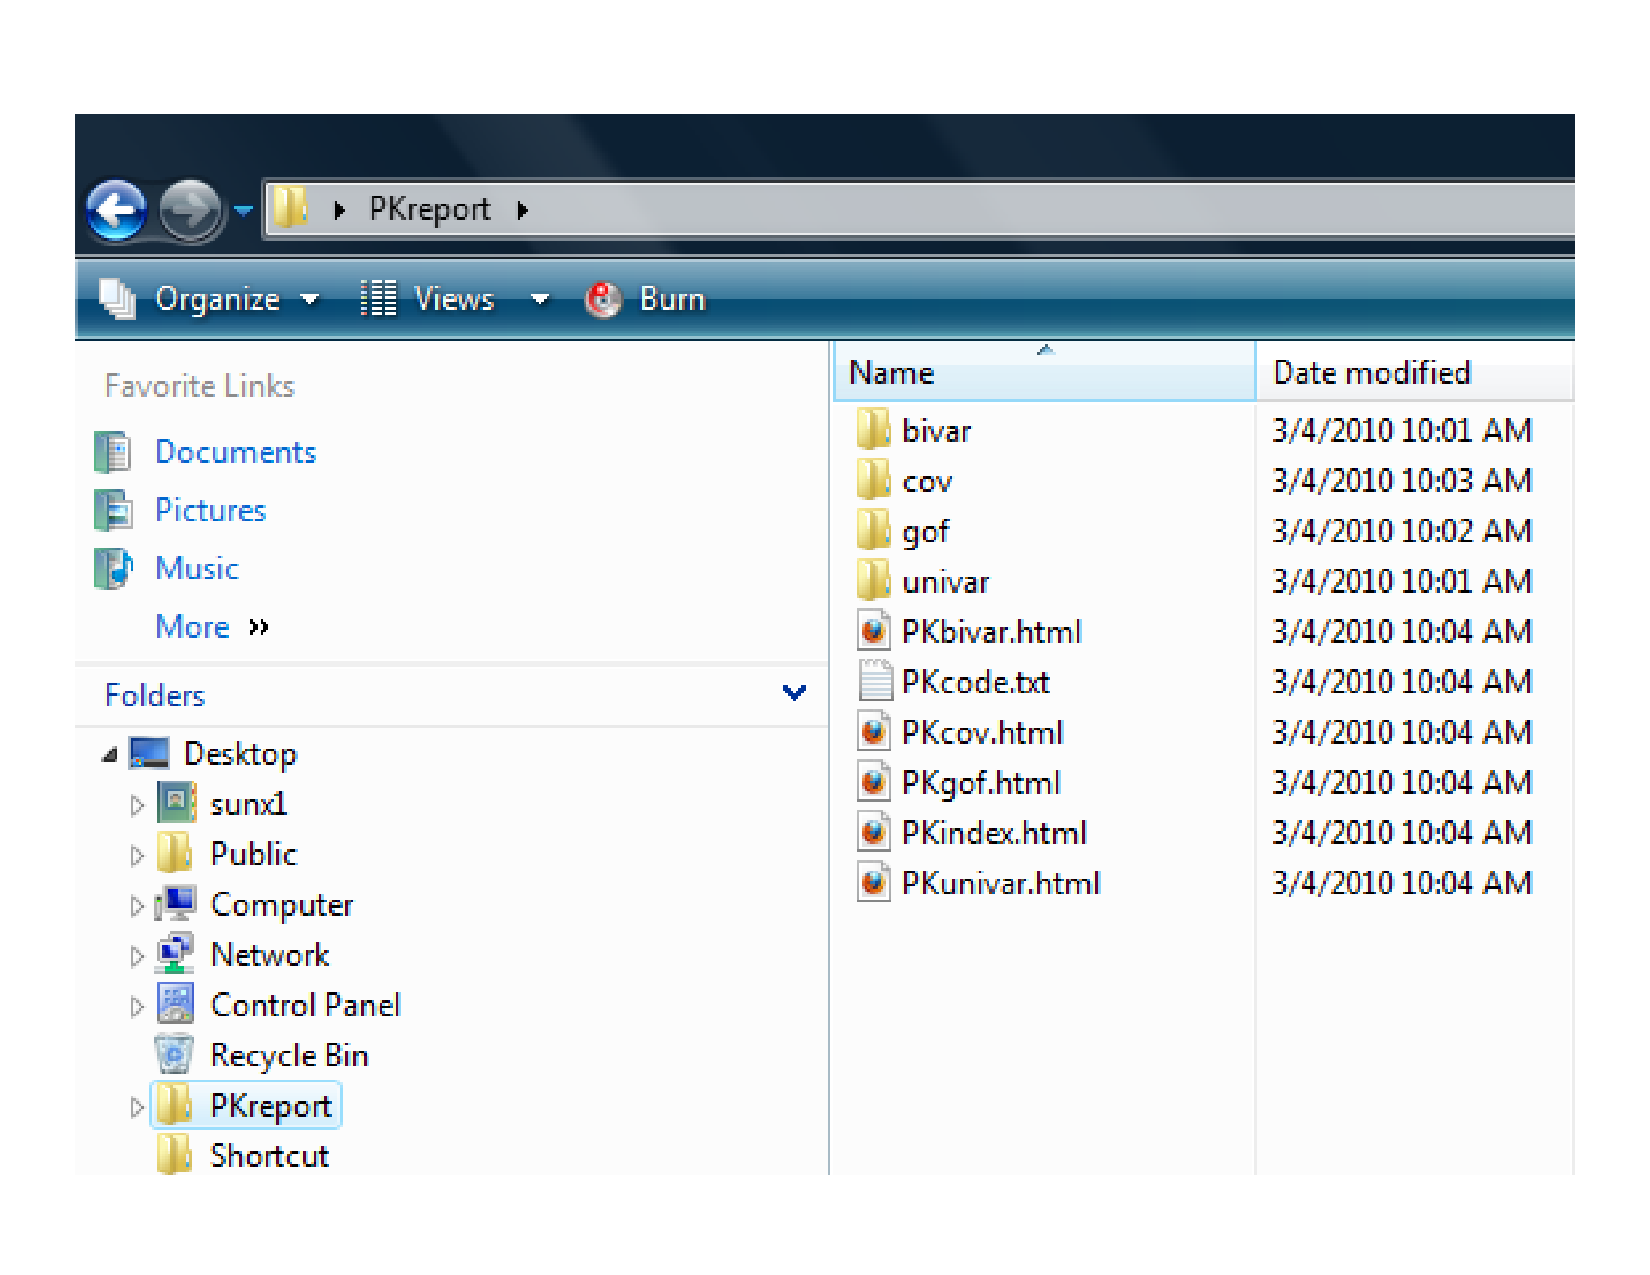
\includegraphics[scale=0.5]{c2_s2_4dir.pdf}
\caption{Archives directories for figures. In this example, \textit{univar} and \textit{bivar} folders match exploratory data analysis; \textit{gof} folder matches goodness of fit plots; \textit{cov} folder matches covariate model diagnostics. These folders contain all related diagnostic figures. \textit{PKcode.text} has all related R scripts for these figures.}
\label{c2_s2_4dir}
\end{figure}

\begin{figure}[h!tb] \centering
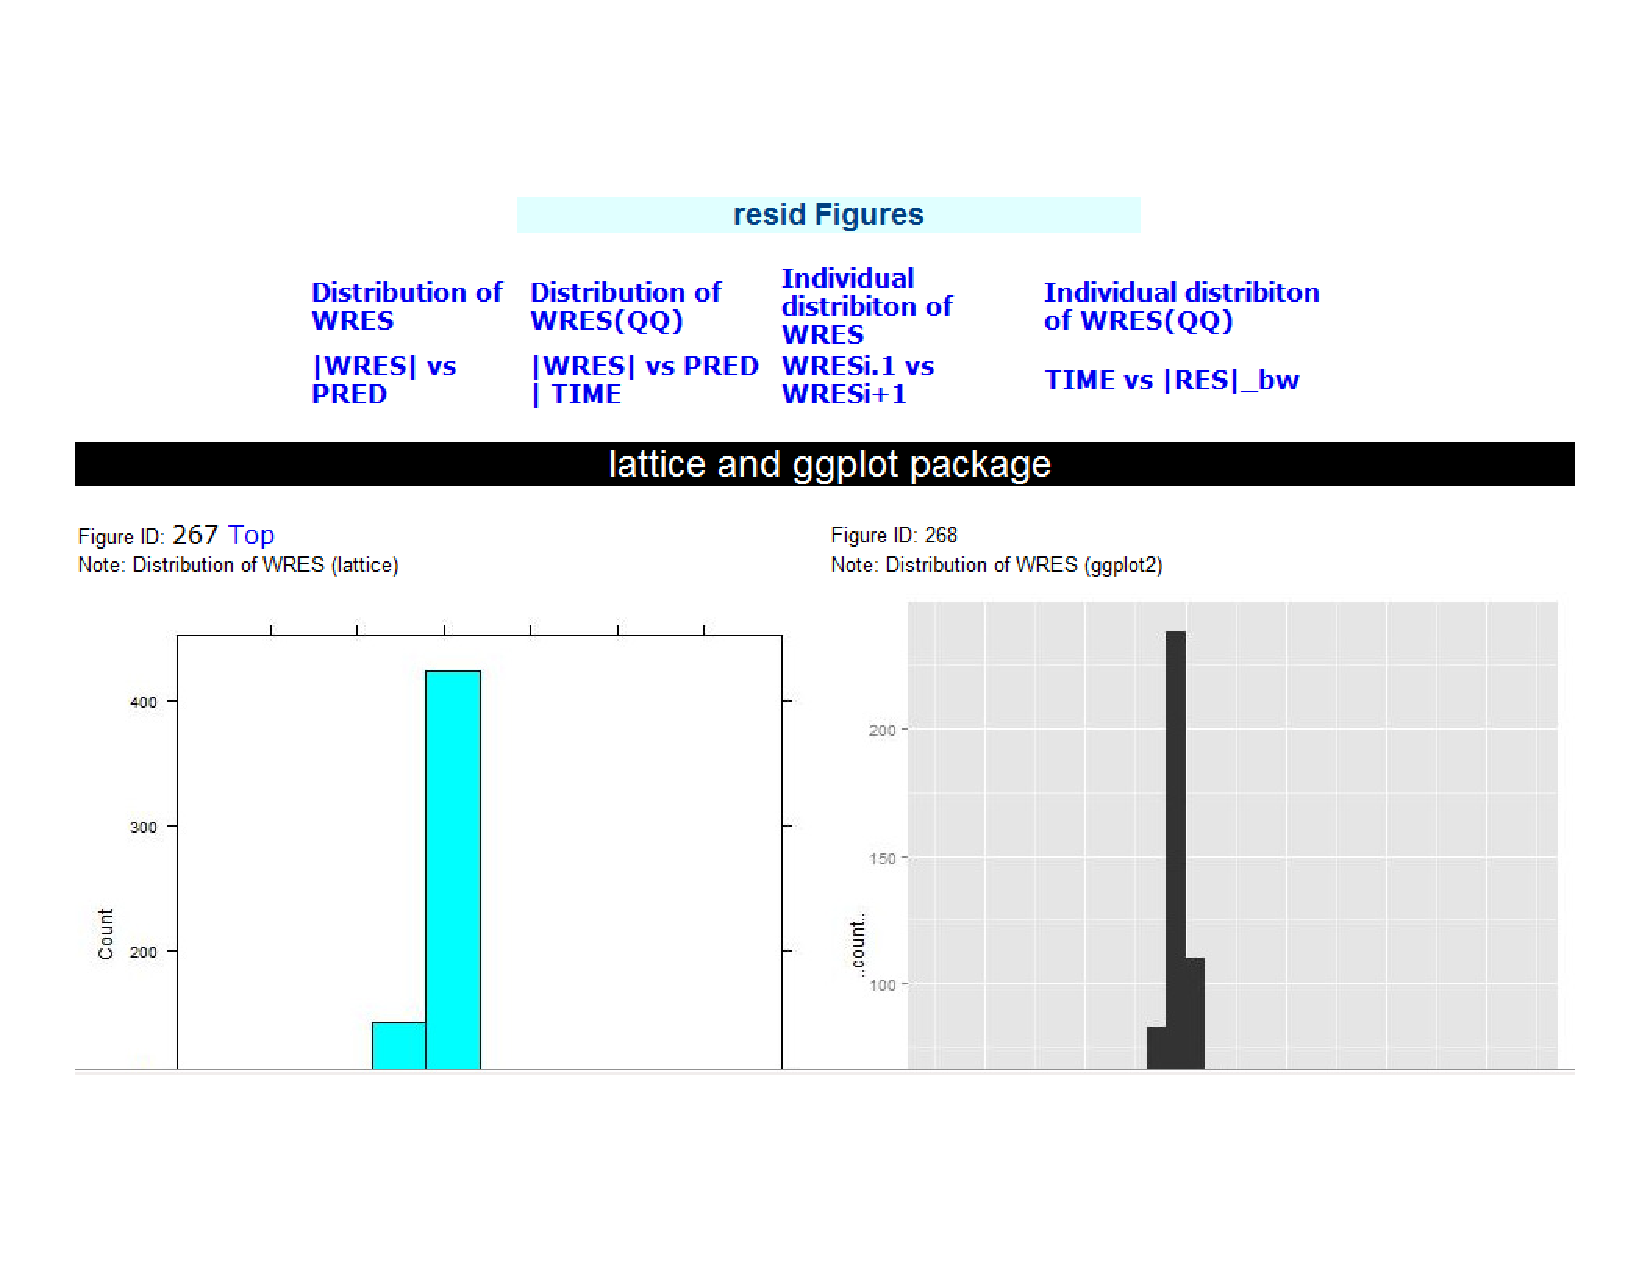
\includegraphics[scale=0.5]{c2_s2_3fig.pdf}
\caption{Figures for residual model diagnostics. A summary list for all figures is on the top. The figure ID matches that in the R code web page, and users can
easily regenerate the figure with this ID. Left figure: histogram for distribution of WRES generated with lattice package. Right figure: histogram for distribution of
WRES generated with ggplot2 package.}
\label{c2_s2_3fig}
\end{figure}

\begin{figure}[h!tb] \centering
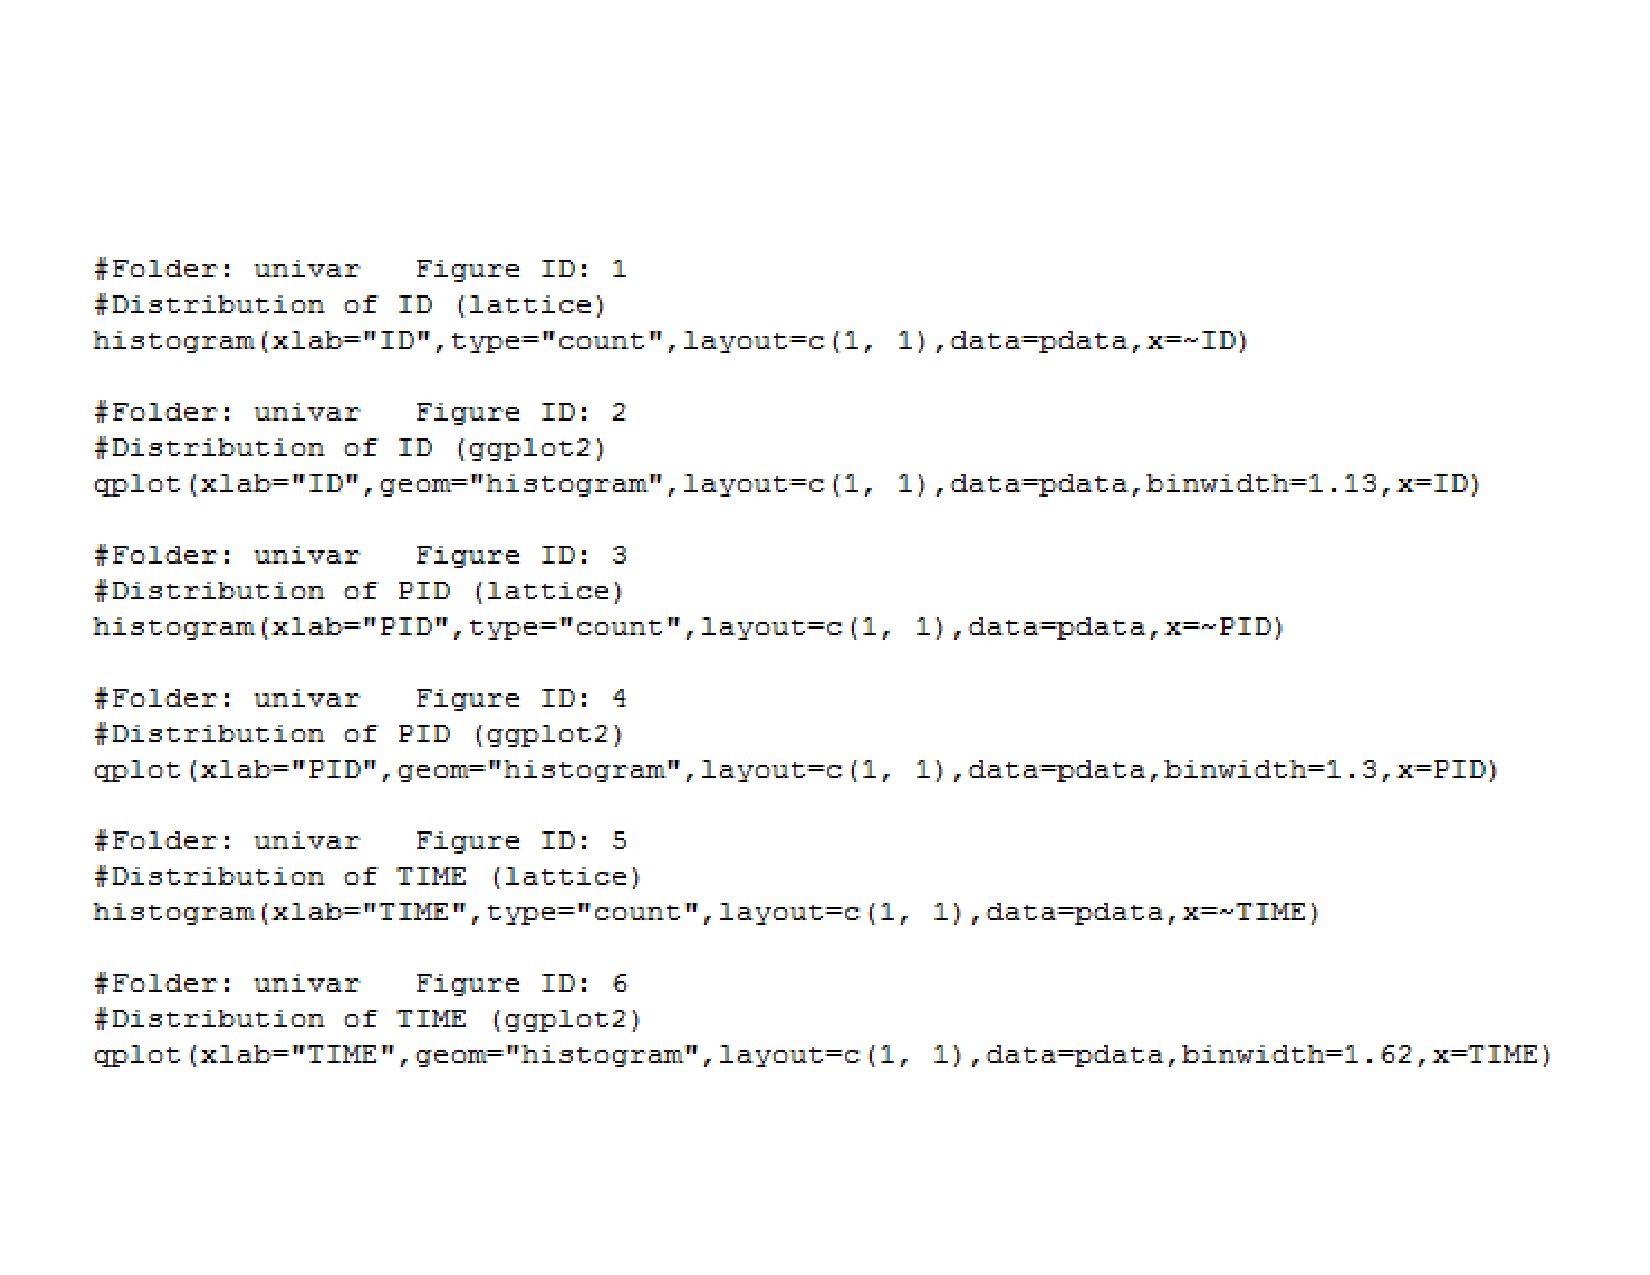
\includegraphics[scale=0.5]{c2_s2_5code.pdf}
\caption{R scripts generated for graphical report. Each R code command includes two comments and one
script. The first comment explains the folder name for this figure
and figure ID matching the graphical report. The second
comment describes the title of the figure.} 
\label{c2_s2_5code}
\end{figure}

\end{document}




